\chapter{绪论}

\section{研究背景与意义}

随着能源输运、轨道交通、周界安防、结构健康监测和地球物理观测等场景对长距离连续监测需求的增加，传统离散式电学传感器在布设密度、供电、抗电磁干扰和维护成本等方面逐渐显现局限。分布式光纤传感以普通通信光纤同时作为传输介质和传感介质，可沿光纤形成连续空间采样通道，并具有无源、抗电磁干扰和便于远距离布设等特点。以瑞利散射为基础的分布式声学传感（distributed acoustic sensing，DAS）能够对沿线动态应变、振动和声学信号进行连续监测，已成为分布式光纤传感的重要技术路线\cite{zhang2021phase_cn,muanenda2018advances,wang2020recent,he2021review,liu2022advances,shang2022research,zhu2022linear}。国内研究已将DAS用于GIS耐压测试、风电地埋电缆、供水管道泄漏和海缆锚害等监测场景\cite{huang2023gis_cn,huang2025cable_thesis,zhang2023pipeline_thesis,zhang2025submarine_cn}，并在语音与脚步等周界振动监测中完成系统实验验证\cite{sun2023voice_cn}，表明该技术正由实验室性能研究向行业应用拓展。

\begin{figure}[htbp]
  \centering
  \subfloat[轨道交通基础设施]{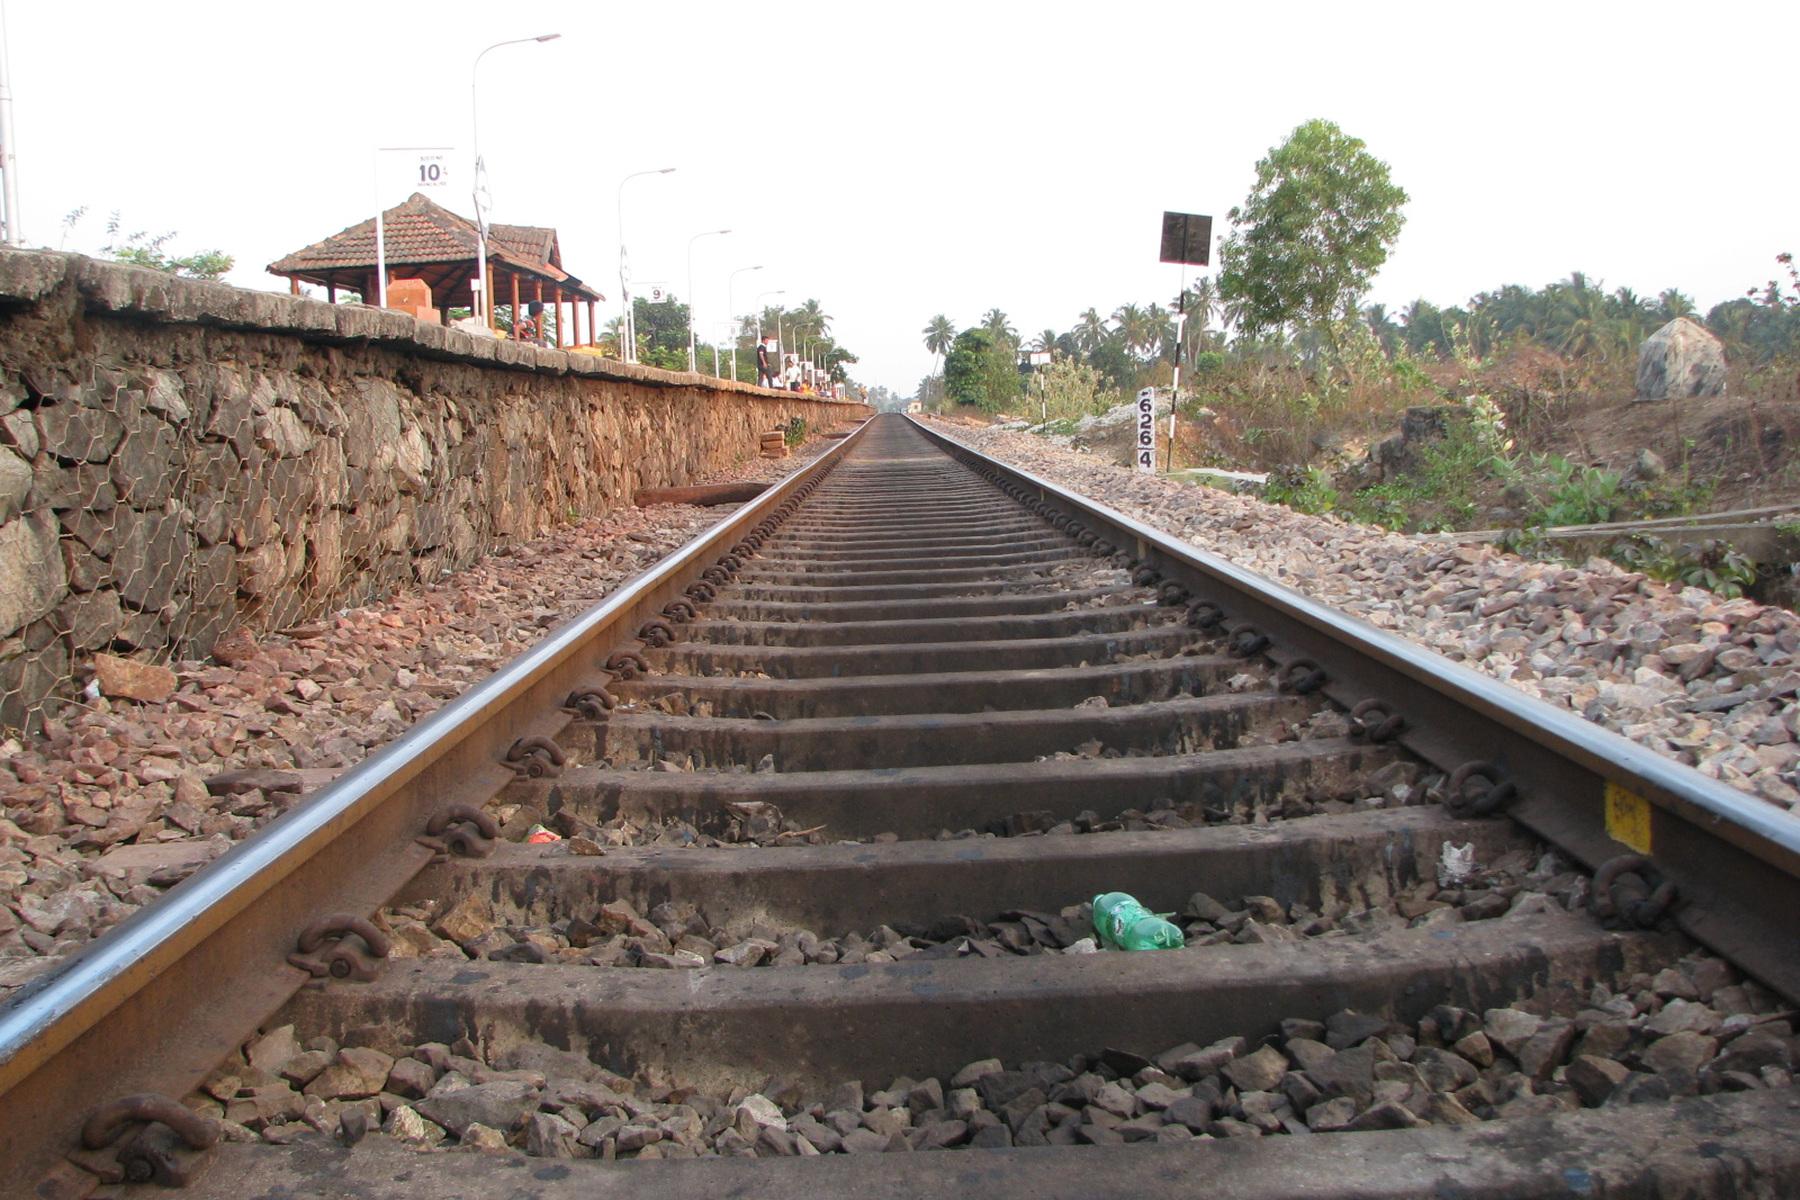
\includegraphics[width=0.315\textwidth]{images/chap1_application_railway.jpg}}
  \hfill
  \subfloat[长距离管线]{
\includegraphics[width=0.315\textwidth]{images/chap1_application_pipeline.jpg}}
  \hfill
  \subfloat[风电设施]{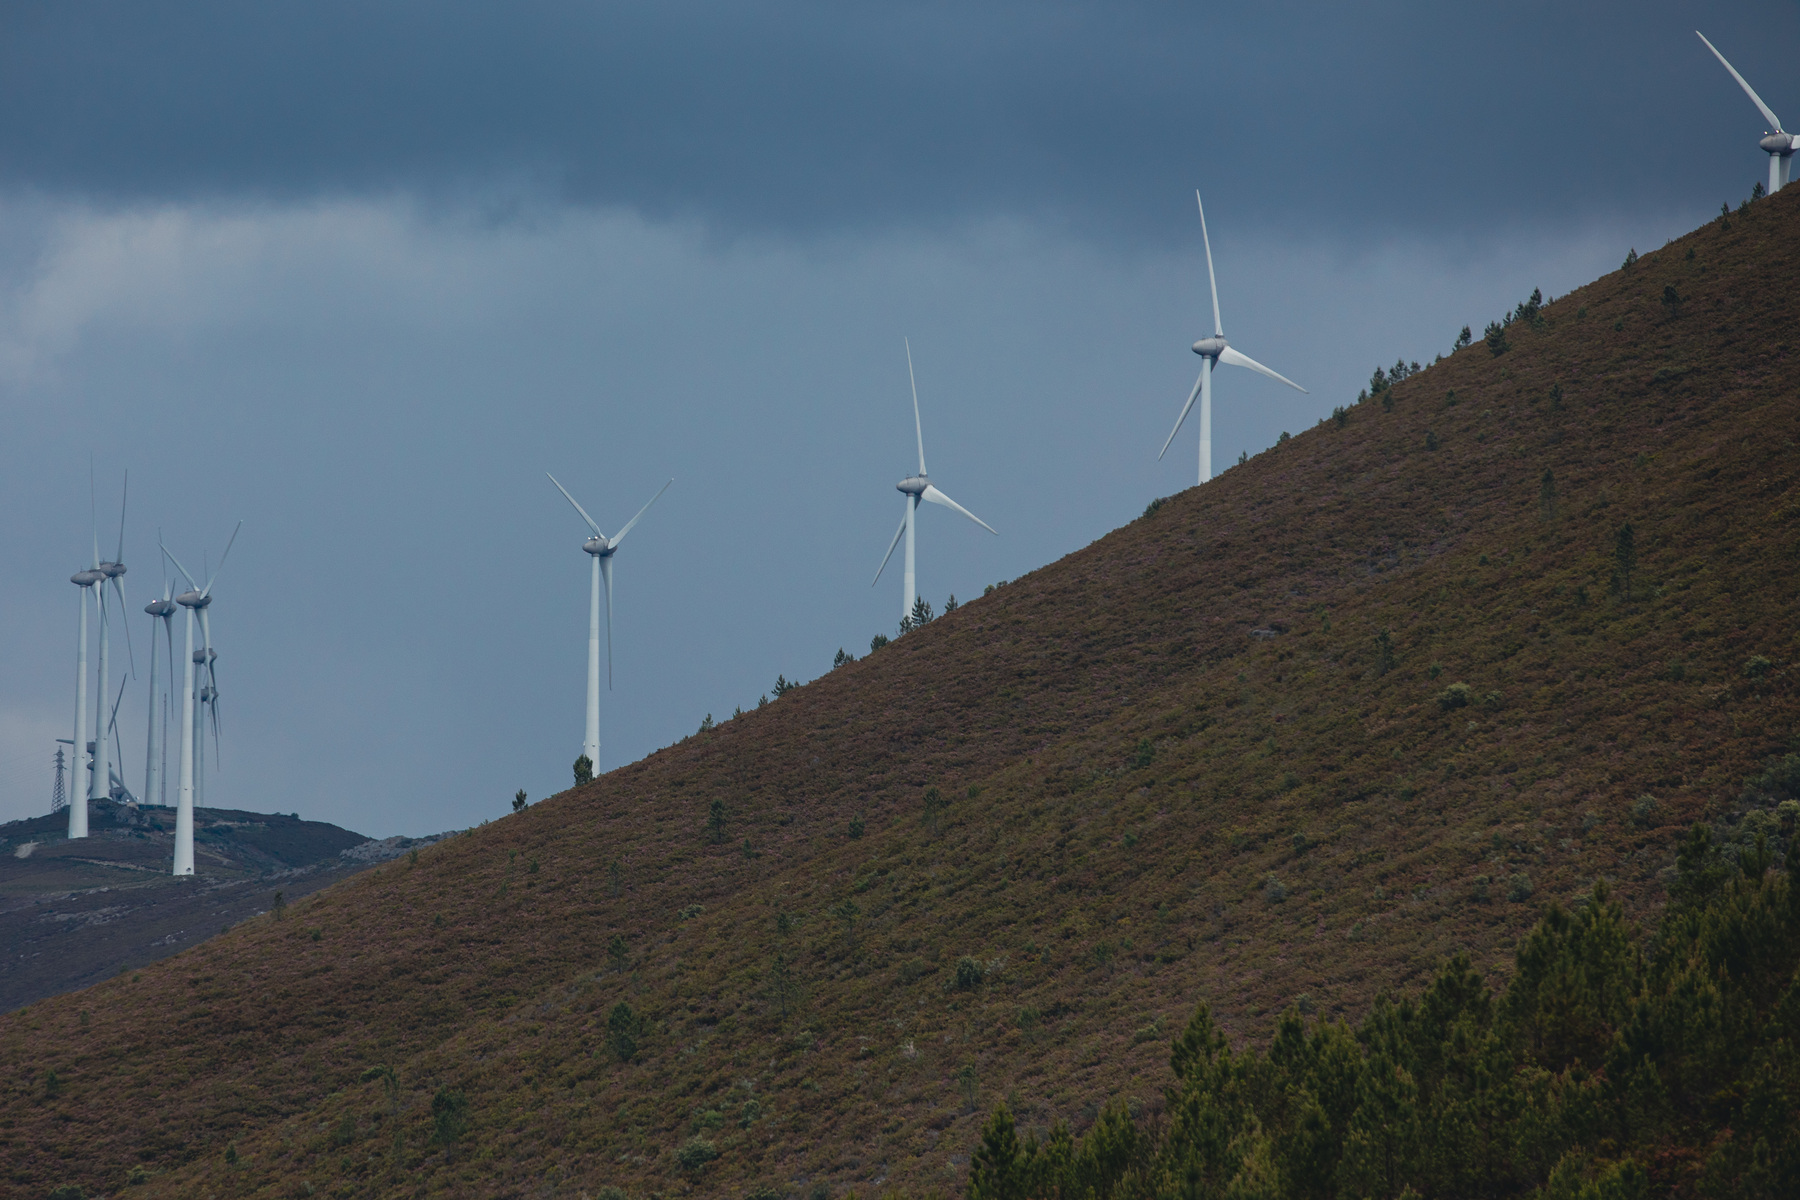
\includegraphics[width=0.315\textwidth]{images/chap1_application_wind.jpg}}
  \caption[DAS典型应用场景实物图]{DAS典型应用场景实物图。照片来源：（a）Shyjuo，CC0 1.0；（b）美国鱼类和野生动物管理局，公有领域；（c）Mussi Katz，CC0 1.0；均经等比例裁剪。图中照片用于说明DAS的潜在布设环境，不代表本文的现场实验。}
  \label{fig:chap1_das_applications}
\end{figure}

图\ref{fig:chap1_das_applications}所示场景在空间尺度、环境条件和目标事件频率方面存在明显差异，但都要求传感链路能够在较长距离上保持连续覆盖，并在复杂背景下稳定恢复局部扰动。因此，DAS研究不仅需要提高单次测量的灵敏度，还需要同时考虑系统体积、长期稳定性、重复装调一致性和现场部署条件。

相位敏感光时域反射（phase-sensitive optical time-domain reflectometry，φ-OTDR）利用窄线宽相干光脉冲在光纤中产生的瑞利后向散射，通过回波到达时间确定扰动位置，并通过散射光场的幅度或相位变化恢复外界动态信息。早期研究验证了相干瑞利散射对应变变化的敏感性\cite{posey2000strain}，随后窄线宽光源稳定性\cite{choi2003stable}、外差相干探测\cite{lu2010distributed}和数字相干接收\cite{pan2011phase}等工作逐步奠定了定量分布式振动测量的系统基础。与只检测回波强度的方案相比，相干接收能够保留复光场信息，为差分相位解调、波形恢复和稳定性分析提供条件\cite{liokumovich2015fundamentals,yang2022digitalized}。

实际DAS性能并不由单一指标决定。脉冲宽度、峰值功率和消光比影响空间分辨率及相邻脉冲之间的背景串扰；光源线宽、频率漂移和非线性传播影响相干性与相位噪声；声光调制器（acousto-optic modulator，AOM）的移频与动态响应决定外差中频和有效门控窗口；偏振态随机演化会造成局部相干衰落；采样率、数字本振、滤波器带宽、差分标距和相位展开方法则共同决定解调结果的连续性\cite{martins2013modulation,ren2016extinction,lu2021detection,lu2022phaseerror,zhong2021frequency,zhao2024frequency,qian2025drift}。因此，发射、传输、接收和数字处理不宜被视为彼此独立的模块，而需要在统一的系统链路中分析。

传统实验平台多由分立光纤器件搭建，便于更换器件和观察中间节点，但连接点较多，系统体积、装调工作量以及重复插拔后的一致性均可能受到影响。近年来，片上调制器、硅光相干接收和混合集成询问器的出现表明，DAS系统正向小型化与集成化方向发展\cite{cheng2023onchip,jin2024integrated,jin2026hybrid}。本文以集成激光二极管--半导体光放大器（laser diode--semiconductor optical amplifier，LD--SOA）光源为基础，将LD--SOA光源、AOM、平衡光电探测器（balanced photodetector，BPD）、偏振分束器（polarization beam splitter，PBS）、$2\times2$耦合器和环形器等器件进行模块级光路集成，形成DAS收发集成光模组。该模组属于器件封装和光路模块级集成，并非将全部功能制作在单一光子芯片上。通过与分立系统开展等条件性能比较，可从光学性能、传感性能、稳定性和工程实现等方面评价集成方案的实际价值。

\section{国内外研究现状}

\subsection{φ-OTDR/DAS技术发展与性能提升}

φ-OTDR/DAS的发展经历了由相干瑞利散射可行性验证、分布式振动定位、定量相位恢复，到性能扩展和工程应用的演进过程。2000年，Posey等利用相干瑞利散射实现光纤应变测量，为通过散射光相位变化感知外界扰动提供了早期实验依据\cite{posey2000strain}。2003年，Choi和Taylor针对φ-OTDR对光源相干性的要求，研究了频谱稳定的掺铒光纤激光器\cite{choi2003stable}。2005年，Juarez和Taylor将偏振判别引入φ-OTDR周界传感，说明回波偏振状态会影响事件检测，并可通过正交偏振观测加以利用\cite{juarez2005polarization}。这一阶段的研究主要解决了相干瑞利散射能否用于分布式扰动感知以及光源、偏振等基本条件问题。

2010年，Lu等采用外差相干探测获得沿光纤分布的振动信息，使φ-OTDR由迹线强度比较进一步发展到相干拍频检测\cite{lu2010distributed}。2011年，Pan等提出基于数字相干检测的φ-OTDR系统，通过数字处理恢复回波幅度和相位信息\cite{pan2011phase}。2013年，Martins等分析了调制不稳定性诱发的相干衰落，指出长距离高功率传输中的非线性效应会限制系统性能\cite{martins2013modulation}。2014年，Wang等采用布里渊放大延伸有效传感距离\cite{wang2014brillouin}。2015年，Liokumovich等建立了静态光纤条件下相干OTDR的系统信号模型\cite{liokumovich2015fundamentals}；同年，Wang等利用时序多频光源拓展系统频率响应\cite{wang2015ultrabroadband}。2016年，Ren等进一步研究有限消光比对系统性能的影响，说明脉冲间残余光会引入相干背景和附加噪声\cite{ren2016extinction}；Masoudi和Newson则从动态应变测量角度总结了不同分布式光纤传感方案的发展\cite{masoudi2016review}。至此，研究重点已从“能否检测振动”转向传感距离、空间分辨率、响应带宽和相位保真度之间的综合权衡。

2018年至2020年，φ-OTDR进入编码、啁啾脉冲和高动态范围测量快速发展的阶段。2018年，Muanenda对φ-OTDR型DAS的系统结构和主要性能提升路线进行了综述\cite{muanenda2018advances}。2019年，Wang等将脉冲编码用于提升DAS性能\cite{wang2019pulsecoding}；Fernandez-Ruiz等利用啁啾脉冲实现分布式声学传感\cite{fernandezruiz2019chirped}，Bhatta等进一步研究了啁啾脉冲条件下的大动态范围分布式应变测量\cite{bhatta2019dynamic}。2020年，Chen等针对弱瞬态信号提出统计检测方法\cite{chen2020transient}，Wang等则系统总结了φ-OTDR在脉冲编码、频率复用、相位解调和应用拓展方面的进展\cite{wang2020recent}。这一时期的国外研究重点由基本系统搭建转向更大动态范围和更高检测能力，国内团队也逐步形成多频发射、脉冲编码和相干解调相结合的研究路线。

2021年以后，研究进一步面向高保真、低采样开销、实时处理和工程应用。2021年，Jiang等提出连续啁啾波φ-OTDR\cite{jiang2021continuous}，Soriano-Amat等采用时间扩展方法降低高速采集压力\cite{sorianoamat2021time}，国内研究则围绕动态应变测量、降噪与信号处理开展系统总结和实验研究\cite{ma2021dynamic_cn,wu2021processing_cn,zhang2021phase_cn,rao2021recent,he2021review}。2022年，Yu等研究欠采样采集架构\cite{yu2022sampling}，Yang等利用数字化相位解调和互相关增强拍频相位恢复\cite{yang2022digitalized}；同期综述进一步将衰落抑制、实时处理和系统工程化列为主要发展方向\cite{liu2022advances,shang2022research,zhu2022linear}。田曼伶的硕士学位论文则围绕φ-OTDR扰动信号分类开展研究\cite{tian2022classification_thesis}。

2023年至2025年，国内研究的应用对象和处理方法继续扩展。2023年，相关工作将DAS用于GIS耐压试验、语音与脚步振动监测以及供水管道泄漏检测\cite{huang2023gis_cn,sun2023voice_cn,zhang2023pipeline_thesis}。2024年，刘念超等研究了基于聚类的振动信号识别方法\cite{liu2024clustering_cn}。2025年，Hu等实现了带衰落抑制的实时DAS系统\cite{hu2025realtime}；刘莹淮和冉玉娇分别围绕瑞利散射分布式振动系统性能优化及动态应变范围提升开展研究\cite{liu2025rayleigh_thesis,ran2025dynamic_thesis}，黄森清和张鸿等则将分布式光纤传感应用于风电地埋电缆和海缆锚害监测\cite{huang2025cable_thesis,zhang2025submarine_cn}。近期偏振衰落综述再次表明，稳定相位恢复仍是限制系统长期运行和现场应用的关键问题\cite{lei2025fading_cn}。总体来看，国内外DAS研究均已由单一振动定位逐步转向复杂链路条件下的定量、实时和长期稳定测量；但不同文献采用的脉宽、光纤长度、标距、带宽和评价指标并不一致，其性能数值不能脱离实验条件直接横向比较。

\subsection{脉冲发射、SOA动态与AOM移频研究}

AOM和SOA的研究起步早于其在DAS系统中的具体应用。1977年，Johnson建立了低衍射效率条件下AOM时间响应的几何光学模型，指出声波传播以及声场与光束的空间重叠共同决定衍射光的建立过程\cite{johnson1977aom}。该工作构成分析AOM声学渡越时间、射频门控和光脉冲完整性的基础。此后AOM逐渐成为外差φ-OTDR中产生稳定频移的常用器件，但早期DAS系统更多关注其标称移频，较少讨论动态门控与采集触发之间的时序关系。

SOA方面，1997年，Mecozzi和M{\o}rk分析了皮秒脉冲引起的SOA增益饱和，揭示载流子耗尽和恢复对脉冲放大的动态影响\cite{mecozzi1997saturation}。2002年，Cao和Cartledge对SOA--MZI波长转换器的强度调制和啁啾特性进行了表征，说明增益变化可通过折射率耦合转化为相位和瞬时频率变化\cite{cao2002characterization}。2003年，Talli和Adams进一步研究了SOA增益动态及多波长工作条件下的载流子响应\cite{talli2003gain}。2010年，Baveja等分析了ASE参与条件下的SOA自相位调制，指出ASE、增益饱和和非线性相位之间存在耦合\cite{baveja2010selfphase}。这些研究确立了“载流子—增益—折射率—相位”动态链条，但其研究对象主要是器件或光通信场景，不能直接等同于SOA在DAS链路中的实验结论。

2015年，Matsuura等通过泵浦—探测实验研究量子点SOA放大引起的啁啾特性，进一步说明输入功率和增益状态会改变输出瞬时频率\cite{matsuura2015chirp}。2021年，Yang等利用色散泵浦—探测光谱观测SOA载流子瞬态\cite{yang2021carrier}；同年，Sutili等在亚纳秒电光开关条件下采用外差后处理表征SOA啁啾\cite{sutili2021chirp}。2022年，Sobhanan等系统总结了SOA载流子速率方程、增益饱和、ASE和相位耦合模型\cite{sobhanan2022soa}。2023年，Connelly等进一步对SOA动态功率和啁啾进行直接表征\cite{connelly2023dynamic}。因此，现有文献能够支持SOA动态可能改变输出相位和外差拍频的机理假设，但直接针对“集成LD--SOA发射链路—DAS拍频—相位解调”传递关系的研究仍较少。

在AOM驱动与DAS时序方面，2022年，于淼等研究AOM驱动和探测脉冲时钟关系对低频相位噪声及系统响应的影响\cite{yu2022lowfrequency_cn}。2024年，雷艳阳等利用宽带声光多频调制降低相干衰落\cite{lei2024broadband_cn}；尚秋峰等采用双AOM外差结构，使本振与传感信号承受相近的频漂并通过正交解调抑制其影响\cite{shang2024dualaom_cn}；Zhang等采用直接数字合成技术提高声光脉冲选择驱动的频率和时序稳定性\cite{zhang2024highprecision}。这些工作表明，AOM不只是提供固定频移，其射频稳定性、声场建立过程和同步关系都会传递到拍频和相位解调结果。因此，在SOA脉冲、AOM射频门控和数据采集之间建立统一时序具有理论与工程依据，但具体提前开启和延迟关闭时间仍须根据实际器件响应测量确定。

\subsection{相干接收、偏振分集与数字解调研究}

相干接收和数字解调是在外差φ-OTDR形成之后逐步发展的。2011年，Pan等采用数字相干检测恢复瑞利回波的幅度和相位，为后续数字下变频和差分相位解调奠定了系统基础\cite{pan2011phase}。2018年，Fu等定量分析I/Q幅度不平衡对相干φ-OTDR的影响，说明实际正交通道误差会直接转化为相位误差\cite{fu2018iq}；同年，Dorize和Awwad将偏振分集与互补编码结合，以降低相干OTDR中的偏振衰落\cite{dorize2018polarization}。2019年，Jiang等提出模拟I/Q解调方案以降低数字处理复杂度\cite{jiang2019analog}，Mompo等则采用周期相干编码和偏振分集接收提升动态应变测量的抗衰落能力\cite{mompo2019distributed}。

2020年，Tu等基于邻域统计抑制φ-OTDR衰落噪声\cite{tu2020fading}；Guerrier等提出相干MIMO传感方法，利用多输入多输出观测提高系统对偏振变化的适应能力\cite{guerrier2020mimo}；Liu等利用双折射估计降低偏振相关噪声\cite{liu2020polarization}。2021年，Zhong等研究Sagnac平衡干涉相位解调\cite{zhong2021sagnac}，并有研究从激光频率漂移角度分析相干φ-OTDR后续扰动测量误差\cite{zhong2021frequency}；Lu和Krebber对检测噪声的影响进行量化，指出低回波SNR会降低相位估计稳定性\cite{lu2021detection}；Cui等通过频谱提取和旋转矢量和抑制干涉衰落\cite{cui2021interference}。同年，国内研究系统梳理了降噪、特征提取和机器学习等信号处理路线，并将MEEMD--HHT用于振动特征提取\cite{tian2021signal_cn,wu2021processing_cn,yu2021meemd_cn}。

2022年至2023年，研究重点由基本相位提取转向误差抑制和计算效率。2022年，Lu和Krebber分析相位误差及解包裹错误抑制方法\cite{lu2022phaseerror}，Yang等基于瑞利后向散射拍频信号的互相关实现数字化相位解调\cite{yang2022digitalized}，Gorajoobi等采用高速偏振旋转器降低偏振衰落\cite{gorajoobi2022polarization}。2023年，Liu等通过空间相移提高相位解调速度\cite{liu2023spatial}，司召鹏等沿距离维采用滑动快速傅里叶变换提取相位\cite{si2023fft_cn}，Cheng等提出子带相移方法抑制衰落\cite{cheng2023subband}，Xie等研究偏振与多频融合条件下的衰落抑制\cite{xie2023fading}；Lu和Thomas则进一步分析相位解调中的噪声性能\cite{lu2023phase}。

2024年至2025年，相干DAS解调进一步面向频偏、实时性和复杂传感链路。2024年，Zhu等研究下采样外差φ-OTDR的噪声性能及参数优化\cite{zhu2024downsampling}，Zhao等提出频率漂移抑制方法\cite{zhao2024frequency}，Xiao等采用信号—核相位噪声补偿改善解调\cite{xiao2024signal}，陈娟等将改进SVD用于频分复用信号降噪\cite{chen2024svd_cn}，Meguellati等则利用多芯、多股光纤结构降低噪声和衰落\cite{meguellati2024noise}。2025年，Zhang等系统分析外差φ-OTDR中频信号的频谱特性及其对解调性能的影响\cite{zhang2025if}，Qian等针对激光相位噪声和频率漂移提出延迟拍频差分相位方法\cite{qian2025drift}，Liu等实现单边带频谱截取与旋转矢量和相结合的实时相位解调\cite{liu2025realtime}。同期中文综述将全保偏光路、探测脉冲偏振控制和接收端偏振分集归纳为主要偏振衰落抑制路线\cite{lei2025fading_cn}。

本文采用PBS双路接收和常规双偏振合成，并结合中心频率、区域、标距和滤波参数进行经验优化。由于尚未提出新的偏振融合或自适应频率跟踪算法，该部分应定位为“接收与解调优化”，不单列为算法创新。其评价重点是：在相同原始数据或相同实验条件下，与单偏振、固定中心频率和默认参数基线比较相位跳变、SNR、频率误差和定位稳定性。

\subsection{DAS系统小型化与收发光路集成研究}

分立DAS光路便于实验室研究，但器件数量和光纤连接点增多会带来体积、插入损耗、偏振敏感性和装调重复性等工程问题，因而系统小型化与光路集成逐渐成为研究方向。2023年，Cheng等报道用于DAS的片上高消光比硅基电光调制器，体现了发射端光子集成在改善脉冲消光比和缩小系统体积方面的潜力\cite{cheng2023onchip}。2024年，Jin等在硅光平台上集成调制发射、双正交和双偏振相干接收功能，并与分立DAS系统开展性能比较，验证了集成询问器用于分布式声学传感的可行性\cite{jin2024integrated}。2026年，Jin等进一步将InP外腔激光器与SOI光子芯片结合，形成混合集成DAS询问方案，表明系统集成正在由单个调制或接收功能向光源、发射和相干接收协同集成发展\cite{jin2026hybrid}。

\begin{figure}[htbp]
  \centering
  \subfloat[多项目晶圆交付的硅光芯片]{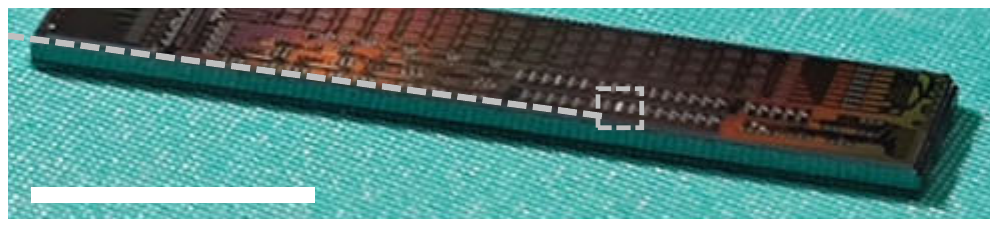
\includegraphics[width=0.56\textwidth]{images/chap1_literature_photonic_chip.png}}
  \hspace{0.04\textwidth}
  \subfloat[封装EOM与商用AOM]{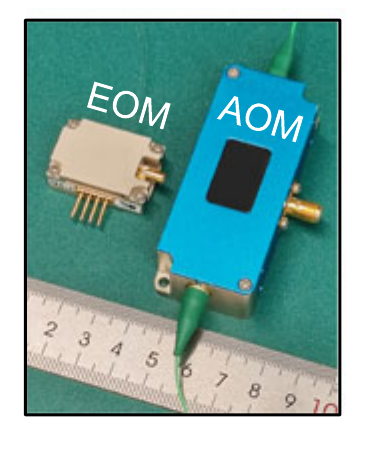
\includegraphics[height=0.23\textwidth]{images/chap1_literature_packaged_eom_aom.png}}
  \caption[DAS集成器件代表性实物图]{：（a）包含耦合微环EOM的硅光芯片；（b）封装EOM与商用AOM的尺寸对比。}
  \label{fig:chap1_literature_hardware}
\end{figure}

图\ref{fig:chap1_literature_hardware}从实物尺度上展示了片上调制器及其封装单元。文献中的照片、器件结构和同条件系统对比共同构成集成化论证，而不是仅以尺寸缩小作为性能结论。这种“工程瓶颈—器件实现—基线比较—传感验证”的论证方式也说明，评价集成方案时必须同时给出光学指标、传感结果和工程指标。

现有文献的集成对象以片上调制器、硅光相干接收器或混合集成询问器为主，与本文将成熟光纤器件封装成收发光模组的实现层级不同。因此，本文不以“片上集成”描述所研制模组，也不直接采用芯片论文的面积、耦合效率或工艺指标作为对照。更合适的比较维度包括：总插入损耗、脉冲峰值与消光比、拍频中心和谱宽、BPD噪声底、双偏振一致性、振动SNR、相位稳定性、扰动定位误差、体积、功耗、接口数量、装调时间以及重复连接后的性能离散度。

分立与集成系统比较还应遵循等条件原则。两套系统应使用相同或可校准的输入光功率、SOA驱动、AOM频率、光纤长度、PZT位置、采样率和数字处理参数；若某些器件型号或内部光程不同，应在表格中明确列出并解释其对结果的影响。这样得到的结论才能回答集成模组究竟改善了工程一致性、长期漂移或传感性能中的哪些方面，而不是仅以体积缩小替代系统性能证明。

\section{本文主要研究内容与技术路线}

围绕集成LD--SOA光源DAS的发射、收发光路集成和相干解调问题，本文保持五章结构开展研究，整体技术路线如图\ref{fig:chap1_research_route}所示。

\begin{figure}[htbp]
  \centering
  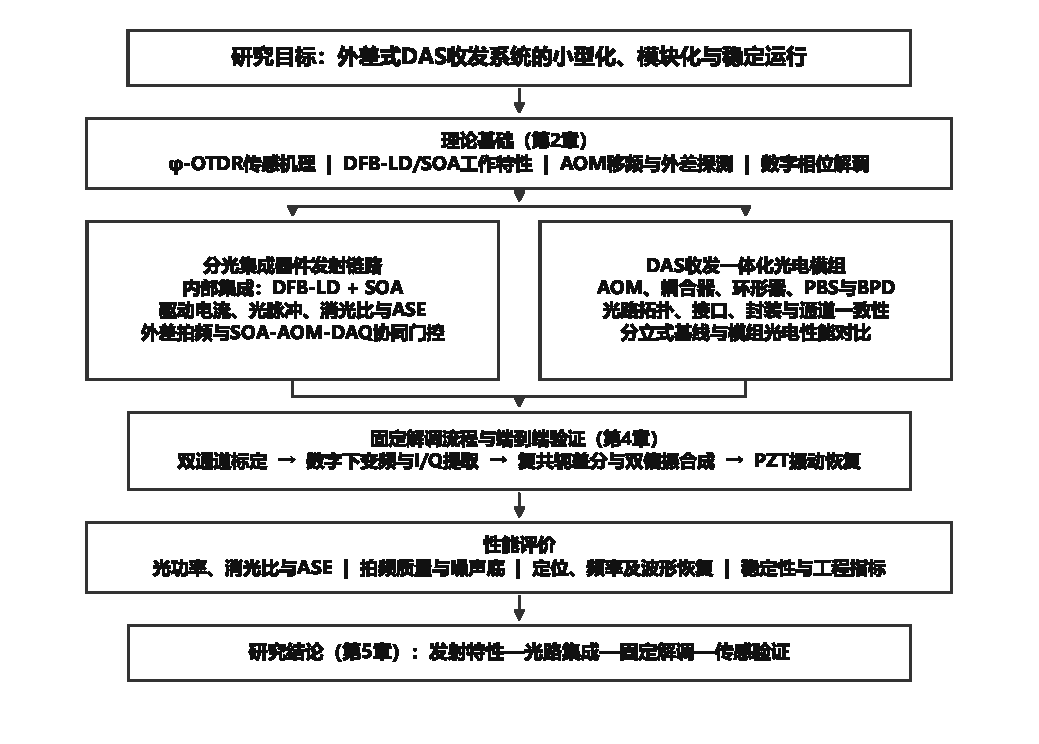
\includegraphics[width=\textwidth]{images/chap1_research_route.pdf}
  \caption{本文研究技术路线}
  \label{fig:chap1_research_route}
\end{figure}

第一章介绍DAS应用背景，综述φ-OTDR、SOA脉冲发射、AOM移频、相干接收、偏振衰落抑制、数字解调以及系统集成化的研究进展，并据此提出本文研究问题。

第二章建立后续实验所需的统一理论模型，包括瑞利后向散射与距离映射、空间分辨率和标距、SOA增益与载流子—折射率耦合、AOM移频和动态响应、外差平衡探测、数字下变频、I/Q相位提取、频率失配和双偏振接收。收发集成光模组本质上是光路结构实现，因此第二章不设置“光模组原理”。

第三章研究集成LD--SOA发射链路及DAS收发集成光模组。首先测试SOA驱动条件对输出脉冲、功率、消光比、ASE和外差频谱的影响；随后给出收发光模组的器件组成、连接关系、封装和接口；最后在等条件下比较分立系统与集成模组的光学、接收、传感及工程性能。SOA载流子动态导致拍频变化的机理只在获得充分排他性实验后作为结论。

第四章研究接收与数字解调优化。通过暗态和断光对照排查电串扰，完成双偏振通道幅值、偏置、极性和时延校准，并比较固定中心频率、实测中心频率及不同区域、标距和滤波参数对振动恢复的影响。该部分定位为系统优化，不宣称新的偏振融合算法。

第五章总结已由文献和实验共同支持的结论，归纳本文工作的适用范围和局限，并对进一步的自动频率跟踪、光电深度集成及现场长距离验证进行展望。

\section{论文主要贡献与研究亮点}

本文围绕集成LD--SOA光源外差式DAS的发射、收发光路集成以及相干接收与数字解调问题展开研究。针对LD--SOA兼具光功率放大与脉冲形成作用所带来的链路耦合、分立光路连接复杂且重复装调一致性不足，以及偏振衰落和解调参数失配影响振动恢复稳定性等问题，本文从发射链路特性与协同门控、收发一体化光电模组实现及等条件评价、偏振分集接收与数字解调优化三个层面构建研究路线。其中，理论分析用于建立瑞利后向散射、SOA载流子--增益--折射率动态、AOM移频、外差平衡探测和差分相位解调之间的联系，并为后续实验选择可观测量、控制变量和评价指标。在此基础上，本文的主要贡献与研究亮点可概括为以下三个方面。

（1）面向不配置EDFA的LD--SOA脉冲发射链路，构建了由器件工作状态、外差拍频质量和相位解调结果组成的系统表征框架，并研究SOA--AOM--DAQ协同门控方法。

集成LD--SOA光源中的SOA同时承担光功率放大和脉冲形成，其驱动电流、脉冲宽度、重复频率、关断偏置及温控状态不仅影响脉冲峰值、消光比、关断漏光和ASE，还可能经由增益与折射率动态传递至外差拍频和相位解调。为避免仅依据单一光功率或频谱现象判断器件机理，本文建立从驱动波形、输出光脉冲、光谱与ASE、拍频中心和谱宽到解调相位的分层观测方法，并通过改变SOA工作状态、固定AOM射频条件以及设置暗态和断光对照，分析器件动态、光路、电串扰和数字处理参数对观测结果的不同贡献。对于SOA工作状态与拍频变化之间的关系，本文将载流子--折射率耦合作为需要通过受控实验检验的机理假设，在排他性证据充分之前不将其直接归因于单一的瞬态啁啾效应。

进一步地，针对SOA载流子建立与恢复、AOM声场传播以及DAQ触发采样均具有有限响应时间的问题，本文研究基于FPGA的SOA--AOM--DAQ协同门控方法。该方法通过设置SOA与AOM射频的提前建立时间、延迟保持时间及DAQ有效采样窗口，使发射脉冲、稳定移频窗口和回波采集区间在统一时间基准下匹配；并以连续射频、命令边沿简单同步和预补偿协同门控作为对照条件，从脉冲完整性、消光比、射频功耗与温升、拍频信噪比、帧间相位稳定性及振动恢复结果等方面评价不同门控策略。该研究将器件动态与系统同步问题纳入同一实验框架，为确定LD--SOA外差式DAS发射链路的稳定工作边界提供依据。

（2）面向分立式DAS光路连接点多、装调复杂和重复连接一致性不足的问题，设计并实现了DAS收发一体化光电模组，并建立分立式光路与集成式模组的等条件评价方法。

本文以20引脚蝶形封装LD--SOA光源模块为发射核心，将AOM、$2\times2$光耦合器、环形器、PBS和BPD等成熟器件按照DAS的发射、回波接收、参考光合束、偏振分集和平衡探测功能进行模块级集成，形成具有统一光电接口的DAS收发一体化光电模组。围绕该模组，本文从功能需求和链路拓扑出发，依次开展器件布局、光纤连接、接口定义、封装、散热、屏蔽和装调设计，并通过逐级测试检查输出光功率、总插入损耗、收发隔离、内部串扰、双偏振通道一致性、拍频质量、热稳定性和重复性。该实现属于成熟光纤器件和光电器件的模块级集成，不将其表述为单片光子集成，也不以体积缩小替代对模组性能的验证。

为分离集成形式与参数优化对系统性能的不同影响，本文设置同参数比较和各自优化后比较两类实验：前者在尽可能保持LD--SOA驱动、AOM射频、传感光纤、BPD、DAQ触发及数字处理参数一致的条件下，对比分立式光路与集成式模组，用于识别集成引入的附加损耗、串扰、噪声和稳定性变化；后者按照相同的优化规则分别确定两种实现形式的合理工作点，用于比较各自可达到的系统性能。评价指标由光链路、隔离与通道一致性、拍频与电噪声、相位解调、端到端振动传感以及体积、功耗、接口数量和装调时间等工程维度共同组成，从而使模组的性能收益、代价及适用范围具有可追溯的对照依据。

\begin{samepage}
（3）围绕DAS收发模组的双偏振输出，形成了偏振分集接收链路标定与数字解调参数协同优化方法，用于提高振动定位和波形恢复的稳定性。

针对实际双偏振接收中可能存在的通道幅值差、直流偏置、极性不一致、时延偏差和电串扰，本文通过暗态、断光和已知输入条件下的对照测量，对两路BPD输出进行幅值、偏置、极性及时延标定，并在相同原始数据或相同实验条件下比较单偏振处理与常规双偏振合成结果。在数字解调环节，本文围绕拍频中心估计、数字本振设置、I/Q误差、有效空间区域、差分标距、空间合并和滤波参数开展协同分析，以固定标称中心频率和默认参数作为基线，从拍频信噪比、相位跳变、有效数据率、振动定位误差、频率恢复误差和波形稳定性等方面评价参数配置的影响。该部分的研究重点是建立与实际模组输出特性相匹配的接收和解调流程，而非提出新的偏振融合算法；其作用在于将模组级光电性能与最终DAS传感结果联系起来，为判断硬件集成后的端到端可用性提供实验依据。
\end{samepage}

总体而言，本文形成了由LD--SOA脉冲发射特性与协同门控、DAS收发光路模块级集成及公平对照、偏振分集接收与数字解调优化构成的三层研究路径。第一部分面向发射质量和统一时序，确定器件工作状态及链路动态的影响边界；第二部分面向系统小型化、接口统一和重复装调一致性，评价模块级集成带来的性能收益与工程代价；第三部分面向模组输出的稳定利用，将光电链路变化落实到振动定位、频率恢复和相位连续性等端到端指标。三者共同服务于集成LD--SOA光源外差式DAS由器件表征、光路集成到传感验证的完整实现，并为后续自动频率跟踪、更高层级光电集成及现场长距离应用提供基础。
